%\documentclass[12pt]{article}

%\usepackage[english]{babel}
%\usepackage[utf8]{inputenc}
%\usepackage{amsmath}
%\usepackage{graphicx}
%\usepackage[colorinlistoftodos]{todonotes}
%\usepackage{amssymb}

%\title{Semi-Inclusive Deep Inelastic Scattering on a longitudinally polarized deuterium target}

\author{S. Pisano}

%\date{\today}

%\begin{document}
%\maketitle

%\begin{abstract}
%Your abstract.
%\end{abstract}

\section{Toward a multi-dimensional mapping of nucleon structure}
%

%PROPOSTA DI FRASE INIZIALE, un po' semplificata e senza questa questione delle dimensioni che mi pare un po' spinosa: 
The Transverse Momentum Dependent distribution functions (TMDs) provide a description of nucleon structure which is complementary to the one that can be obtained measuring Generalized Parton Distributions: the latter describe the correlation between the longitudinal momentum and the transverse position of the parton, while the former encode both the longitudinal and the transverse momenta of the parton. 
%
%(Complementary to the $2+1D$ mapping of nucleon structure encoded in the Generalized Parton Distributions, that describe the correlation of the parton transverse position to its momentum fraction, there is the $3D$ description of the nucleon dynamics, that encode both the longitudinal and transverse distribution of parton momenta and it is implemented in the Transverse Momentum Dependent distribution functions (\textbf{TMD}).)
Thus, the TMDs share with the GPDs the dependence on the parton longitudinal momentum fraction, providing the additional information on its tranverse momentum $k_T$. 
The TMDs can be accessed through the semi-inclusive electroproduction of hadrons (\textbf{SIDIS}), \textit{i.e.} the process where an electron scatters off a nucleon producing a hadron in the final state. In an intuitive picture, the final hadron carries information on the original dynamics of the struck quark, so that mapping the hadron kinematics provides information on the parton motion inside the nucleon.
In the SIDIS cross section different structure functions (\texttt{SF}) are introduced, each being accessible through specific combinations of the polarizations of beam and target.
Any SF contains two non-perturbative objects: the TMDs, encoding the parton dynamics in the nucleon, and the so-called Fragmentation Functions (\textbf{FF}), that describe the transition from the partonic degrees of freedom to the hadronic ones, \textit{i.e.} the hadronization process.
FFs and TMDs are coupled in a convolution integral over the quark transverse momentum, making the final TMD extraction model dependent through the assumptions on the (not measurable) $k_T$ dependence.\\

At leading twist, the parton dynamics is described by eight \textbf{TMDs}, each one related to a specific combination of parton/hadron polarization, as shown in Table~\ref{tab::tmds}. 
The diagonal elements of the table are the momentum, the longitudinal and transverse spin distributions of partons, and represent well-known parton distribution functions related to the square of the leading-twist, light-cone wave functions. Off-diagonal elements require non-zero orbital angular momentum and are related to the overlap of light-cone wave functions with $\Delta L \neq 0$ ~\cite{Ji:2002xn}.  The parton distributions $f_{1T}^\perp$ and $h_1^\perp$ represent the imaginary parts of the corresponding interference terms, while the functions $g_{1T}$ and $h_{1L}^\perp$ represent their real parts. The TMDs $f_{1T}^\perp$ (chiral-even) and $h_{1}^\perp$ (chiral-odd) are known as the Sivers and Boer-Mulders functions, respectively~\cite{Sivers:1990fh,Anselmino:1998yz,Brodsky:2002rv,
Collins:2002kn,Ji:2002aa,Belitsky:2002sm}. They describe unpolarized quarks in the transversely polarized nucleon and transversely polarized quarks in the unpolarized nucleon respectively. 
They vanish at tree-level in a $T$-reversal invariant model ($T$-odd) and can only be non-zero when initial or final state interactions cause an interference between different helicity states. These functions parametrize the correlation between the transverse momentum of quarks and the spin of a transversely polarized target or the transverse spin of the quark, respectively. They both require orbital angular momentum, as well as non-trivial phases from the final state interaction, that survive in the Bjorken limit.\\
%(Therefore, TMDs describe the correlations among the spins and the momenta of the partons and the hadron.) FORSE QUESTA FRASE ORA NON SERVE.
%
% TMD table
\begin{table}
\centering
\begin{tabular}{l|c|c|r}
$N/q$ & U                 & L        & T                 \\\hline\hline
U     & $f_1$             &          & $h_1^{\perp}$     \\\hline
L     &                   & $g_1$    & $h_{1 L}^{\perp}$ \\\hline
T     & $f_{1 T}^{\perp}$ & $g_{1 T}$ & $h_1$ $h_{1 T}^{\perp}$\\\hline\hline
\end{tabular}
\caption{\label{tab::tmds} Leading-twist Transverse Momentum Distributions. Different rows and columns correspond, respectively, to different quark and nucleon polarization states.}
\end{table}
%
%
As for the GPDs, also for the TMDs CLAS12 foresees a comprehensive  program, including measurements of different observables with different targets and polarization degrees of freedom. 
%QUI SECONDO ME STA BENE LA PARTE SUL PERCHE' FACCIAMO PROTONE E DEUTERIO.
%QUESTA FRASE NON E' MOLTO LEGATA ALLA PRECEDENTE. FORSE LA PARTE SU CLAS12 VA BENE ALLA FINE DELL'INTRODUZIONE.
Furthermore, the detection of different hadron channels allows to tag the flavor of the struck quark, opening the avenue to a deeper understanding of the nucleon content and on the hadronization mechanism.\\
%E LE TARGET DIVERSE COSA DANNO? LO CHIEDO PERCHE' A ME NON E' CHIARO, NON STO FACENDO UNA DOMANDA RETORICA.\\
%
\subsection{Scientific case}
%
In the experiment proposed here, which requires to extend by 50 days the already approved experiment E12-09-009, the simultaneous presence of a longitudinally polarized beam and a longitudinally polarized target allows the measurement of longitudinal target and double-spin asymmetries ($A_{UL}$ and $A_{LL}$ respectively). In these asymmetries, a number of relevant TMDs appear:
%
\begin{equation}
\sigma_{UU} \propto F_{UU} \propto f_1(x, k_\perp) D_1(z_h, p_\perp) 
\end{equation}
%
\begin{equation}
\sigma_{UL} \propto F_{UL} \propto h_{1L}(x, k_\perp) H^\perp_1(z_h, p_\perp) 
\end{equation}
%
\begin{equation}
\sigma_{LL} \propto F_{LL} \propto g_{1L}(x, k_\perp) D_1(z_h, p_\perp) 
\end{equation}
%
%
where $z=P_1\dot{P_h}/P_1\dot{q}$ is the fraction of the virtual photon energy carried by the final hadron, $k_\perp$ and $p_\perp$ are the quark transverse momenta before and after the interaction with the virtual photon, $P_1$ and $P_H$ are the four momenta of the initial nucleon and the observed final-state hadron, respectively. 
The unpolarized ($D_1$) and polarized ($H^\perp_1$) fragmentation functions depend in general on the transverse momentum of the fragmenting quark.
For the longitudinal target spin asymmetry, the leading-twist modulation is a $\sin2\phi$ moment, that provides access to the Kotzinian function $h_{1 L}^{\perp}$, \textit{i.e.} the \texttt{T-even} counterpart of the Boer-Mulders function. 
The same distribution function is also accessible in double-polarized Drell-Yan production.
It describes the correlations of the tranverse spin and momentum of quarks in a longitudinally polarized nucleon and, being an off-diagonal element, requires a non-zero orbital angular momentum to be non vanishing.
%
Moving beyond the leading-twist approximation, a second, \texttt{twist-3} modulation is expected in $A_{UL}$. It can be accessed as a $\sin\phi$ moment, and provides access to a combination of different TMDs and FFs. The simultaneous extraction of leading and higher-twist modulations in the observables at the CLAS12 kinematics will play an essential role in sizing effects beyond the leading twist. The CLAS12 kinematic coverage, indeed, is characterized by a $Q^2$ value laying in a region where possible higher-twist phenomena are still active.\\ %An example is the measurement performed at 6 GeV (citare misura di Harut), that, for the first time, reported a non-zero $\sin2\phi$ moment for $A_{UL}$, differently from the previous measurement by HERMES that found a $A_{UL}^{\sin2\phi}$ consistent with zero.
%
Double-spin asymmetry $A_{LL}$ is proportional to the diagonal TMD $g_1(x, k_\perp)$, that reduces to the 1D helicity distributions once the $k_\perp$ dependence is integrated out. Measurements of the $P_T$ dependence of $A_{LL}$
for different hadron channels will provide access to widths in transverse momentum for different flavors.
%
%
Also interesting is the exploration of the Collins mechanism, encoded in the FF that appears coupled to $h_{1 L}^{\perp}$ in $A_{UL}$.
In the so-called $u$-quark dominance scenario, where the fragmentation is led by the dominant flavor in the nucleon, similar results would be expected from pion and kaon fragmentation. However, the available results from HERMES (and COMPASS) 
on kaons do not confirm this scenario, with a signal for positive kaons being larger than for pions, while for negative kaons they are compatible. The kaon signals are a challenge for the present understanding of the underlying physics processes. Detailed studies require disentanglement of the different contributions, which is possible only
with high-precision mapping of the kinematical dependences.
The surprising and controversial pattern of azimuthal asymmetries for kaons is an
indication of a non trivial role of the sea quarks in the nucleon, or of a peculiar behaviour
of the fragmentation mechanism in the presence of strange quark.\\

In order to shed light on the hadronization mechanism, a high-precision mapping of the kinematic dependences, in conjuction with a excellent hadron identification will be mandatory. Furthermore, measurements for \texttt{different hadron channels} (that allow to tag the flavor of the decaying quark) on \texttt{different targets} will allow to extract different combinations of TMD and favored/unfavored fragmentation functions.
%
%\todo[inline, color=green!40]{Flavor separation.}
%
%
\subsection{Channel selection and data analysis}
\label{sec::channel_sel}
%
%
The process of interest is the semi-inclusive electroproduction of a single hadron, \textit{i.e.}
%
\begin{equation}
e (k) d (p) \Rightarrow e (k') h (P) X
\end{equation}
%
%
% SIDIS process
\begin{figure}
\centering
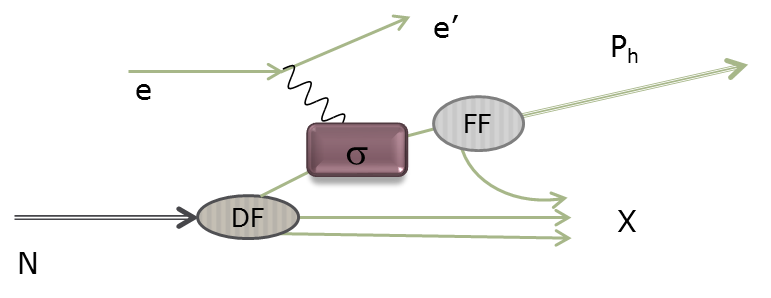
\includegraphics[width=0.85\textwidth]{sidis/sidis_drawings.png}
\caption{\label{fig::sidis} Semi-inclusive electro-production of a hadron $h$. The box labeled $\sigma$ represents the hard part of the cross-section, described by quantum electrodynamics. The soft, non-perturbative blob represents the distribution functions (DF) that describe the dynamics of the partons in the nucleon (DF=TMD in the SIDIS case), while FF represent the hadronization of the struck quark to the final hadron.}
\end{figure}
%
The electron scatters off the deuterium through the exchange of a virtual photon. The latter interacts with one of the nucleon partons (a quark, in the CLAS12 kinematics) that eventually hadronizes through a fragmentation process producing the hadron $h$ in the final state.\\
Particle identification will mainly exploit the forward detectors of CLAS12. Electrons will be identified through the calorimeter system (PCAL + EC), the time of flight and the high-threshold Cherenkov counter, and the tracking information will come from the Drift Chambers.
Charged pions will be identified through the combination of tracking, time-of-flight and Cherenkov counter information. The neutral pions will be reconstructed through their two-photon decays, exploiting information from the calorimeters.
In order to get a reliable particle identification in the kinematical region of interest, the use of the \texttt{RICH} detector will be mandatory, being the complementary PID system of CLAS12 not efficient in the kinematics proper of SIDIS hadrons (see, e.g., Fig. \ref{fig::kaon_p_theta}).
%
%
% kaon kinematics
\begin{figure}
\centering
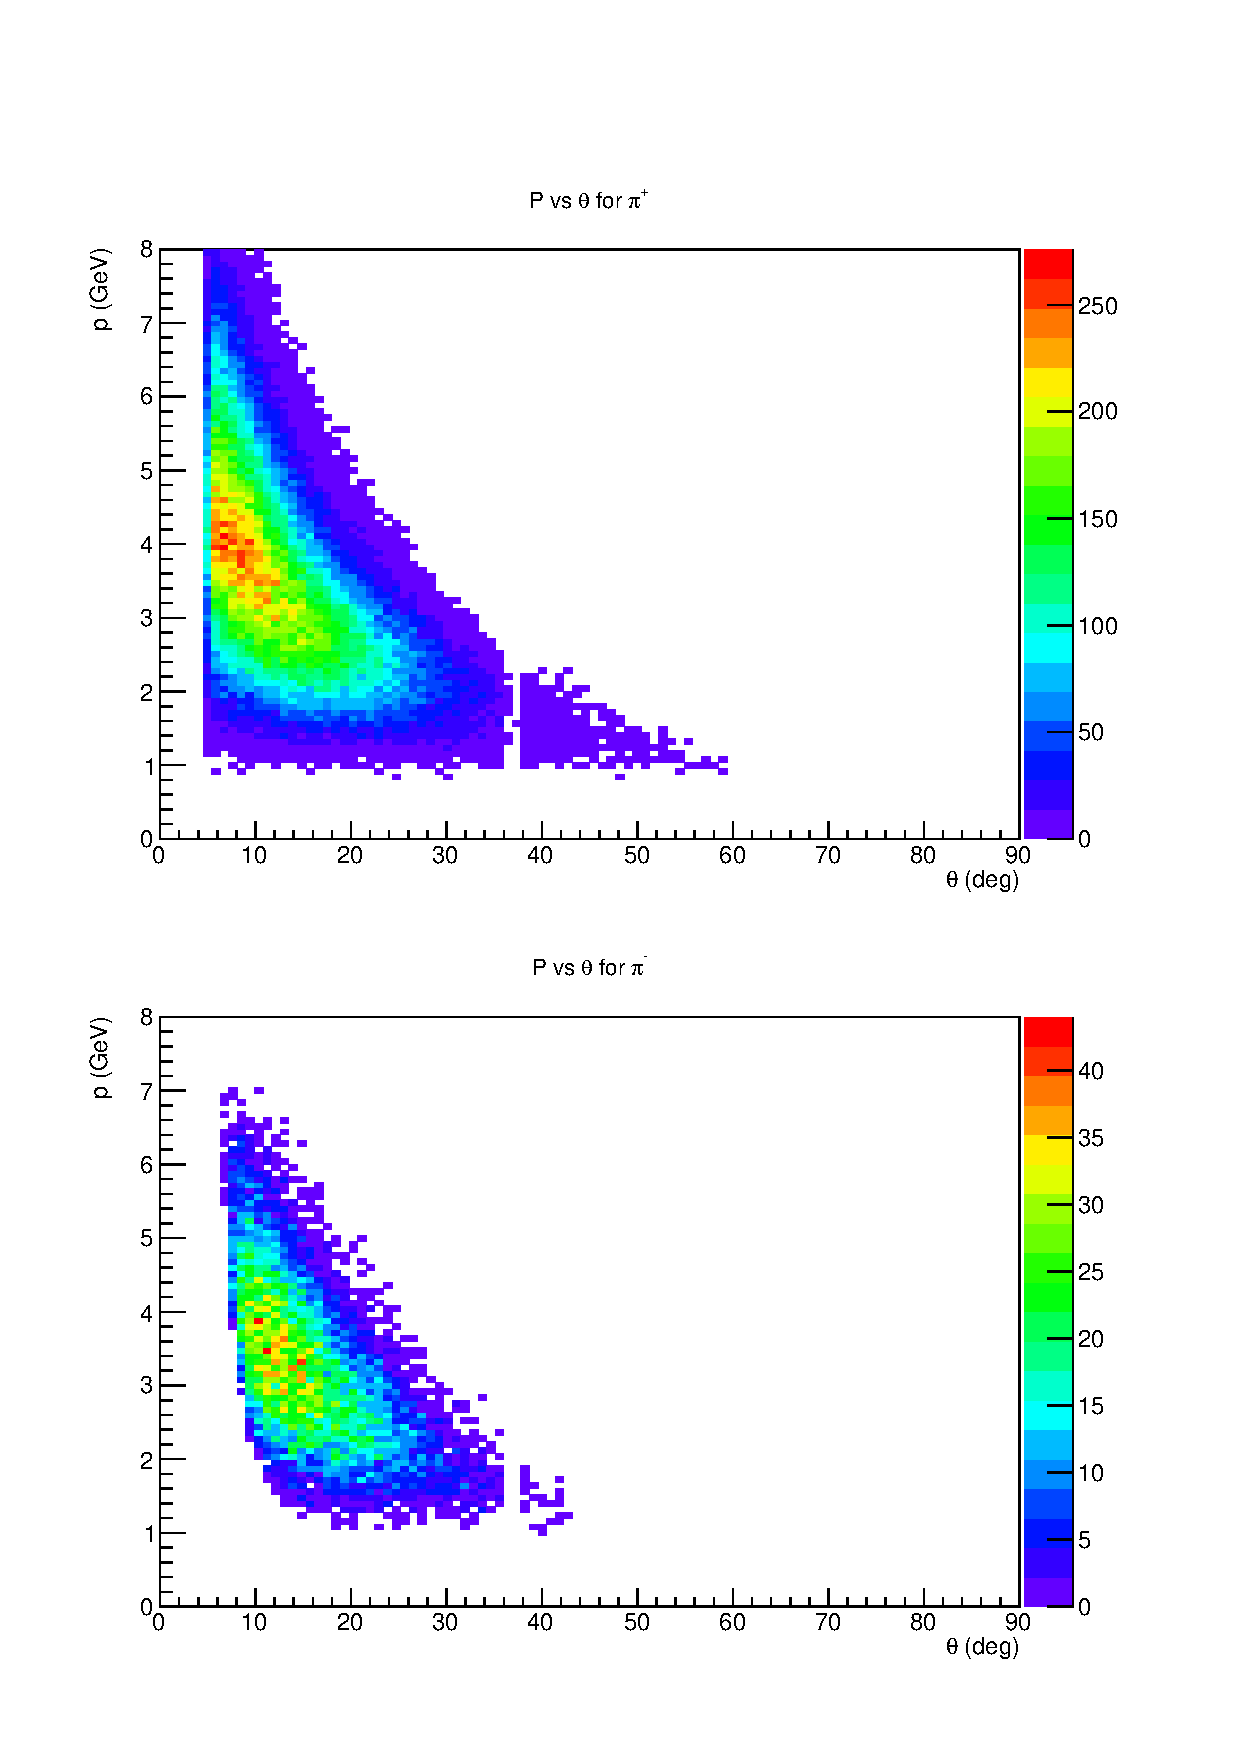
\includegraphics[width=0.85\textwidth]{sidis/kaon_p_theta.pdf}
\caption{\label{fig::kaon_p_theta} P \textit{v.s.} $\theta$ for positive (top plot) and negative (bottom plot) kaons. The distributions are produced by selecting SIDIS kaons as described in Sec. \ref{sec::channel_sel}.}
\end{figure}
%
%
The final sample will be selected applying deep-inelastic cuts ($Q^2>$ 1 GeV$^2$, $W>$1 GeV) to select a regime where scaling is already at work and to exclude possible contributions from nucleon resonances. 
Contamination from target-fragmentation hadrons will be removed by applying a cut on the fraction of the virtual photon energy carried by the hadron, $z$, that will also remove contributions from the exclusive channels. At 6 GeV the typical $z$ cuts were 0.4 $<z<$ 0.7, the lower one removing contamination from delta-mediated decays and the higher one from residual exclusive events.
As an example, in Fig.~\ref{fig::mx} the distribution of $m_{e^-\kappa^+X}$ is shown as a function of the $z$ of the positive kaon. The contribution from exclusive events, peaking at the nucleon mass, appears clearly visible in the high-$z$ region and will be removed through the above-mentioned upper cut on $z$.\\
%
%
%
% SIDIS process
\begin{figure}
\centering
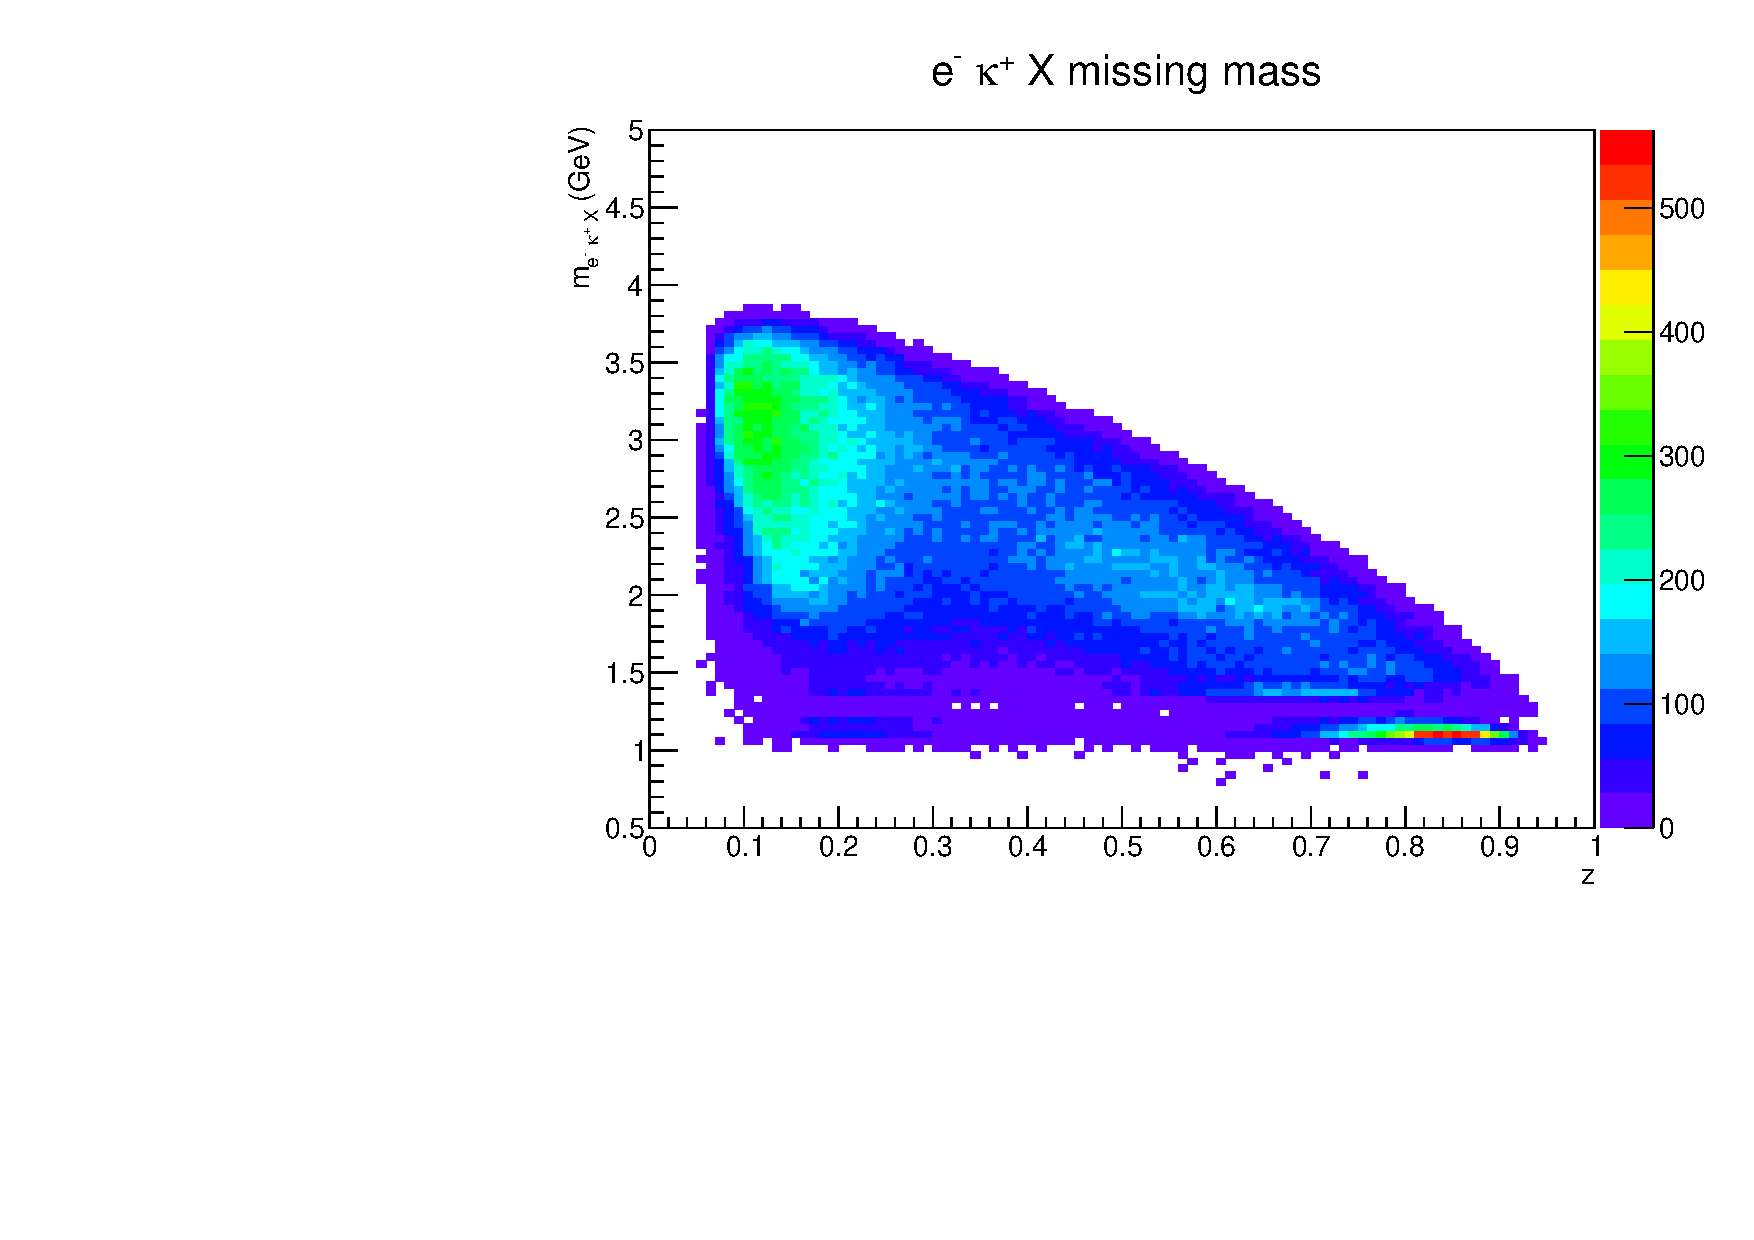
\includegraphics[width=1.0\textwidth]{sidis/mmElKaPX.pdf}
\caption{\label{fig::mx} Distribution of the $e^-\kappa^+X$ missing mass as a function of $z$ of the positive kaon. The contribution from the exclusive peak appears clearly in the high-$z$ region.}
\end{figure}
%
%
The relevant variables for mapping single and double spin asymmetries are the ones describing the electron kinematics, $(x_B, Q^2)$, the hadron tranverse momentum $P_T$ and the fraction of the virtual-photon energy carried by the hadron $z$. The latter appear in the fragmentation functions, and are proper to the hadronization process.
Distributions on $p_T$ for positive and negative pions are shown in Fig. \ref{fig::phi_pt_kpm}: left plot refers to the positive kaons, while right plot to negative.
%Furthermore, TMDs and FFs appear in the observables coupled through a convolution integral over the quark tranverse momentum $k_T$. 
In order to extract the relevant azimuthal modulations, the asymmetries will be measured as a function of the angle $\phi$, formed by the leptonic and hadronic planes, shown in Fig. \ref{fig::phi_angle} and defined according to the Trento Conventions.
%
%
% phi angle
\begin{figure}
\centering
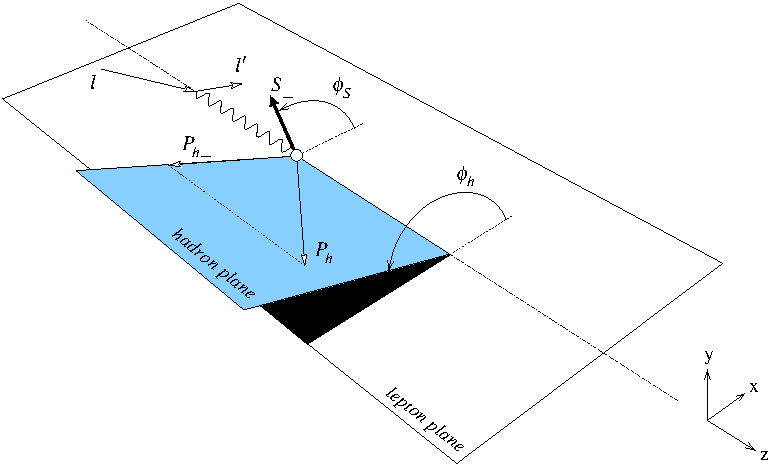
\includegraphics[width=1.0\textwidth]{sidis/anglestrento.pdf}
\caption{\label{fig::phi_angle} Definition of the angle $\phi$, formed by the leptonic and the hadronic planes.}
\end{figure}
%
The acceptance in $\phi$ for charged kaons is shown in the two upper plots of Fig. \ref{fig::phi_pt_kpm}. The left plot shows the $\phi$ distribution for positive kaons, while the right one refers to negative kaons.
%
%
% phi acceptance for kaons
\begin{figure}
\centering
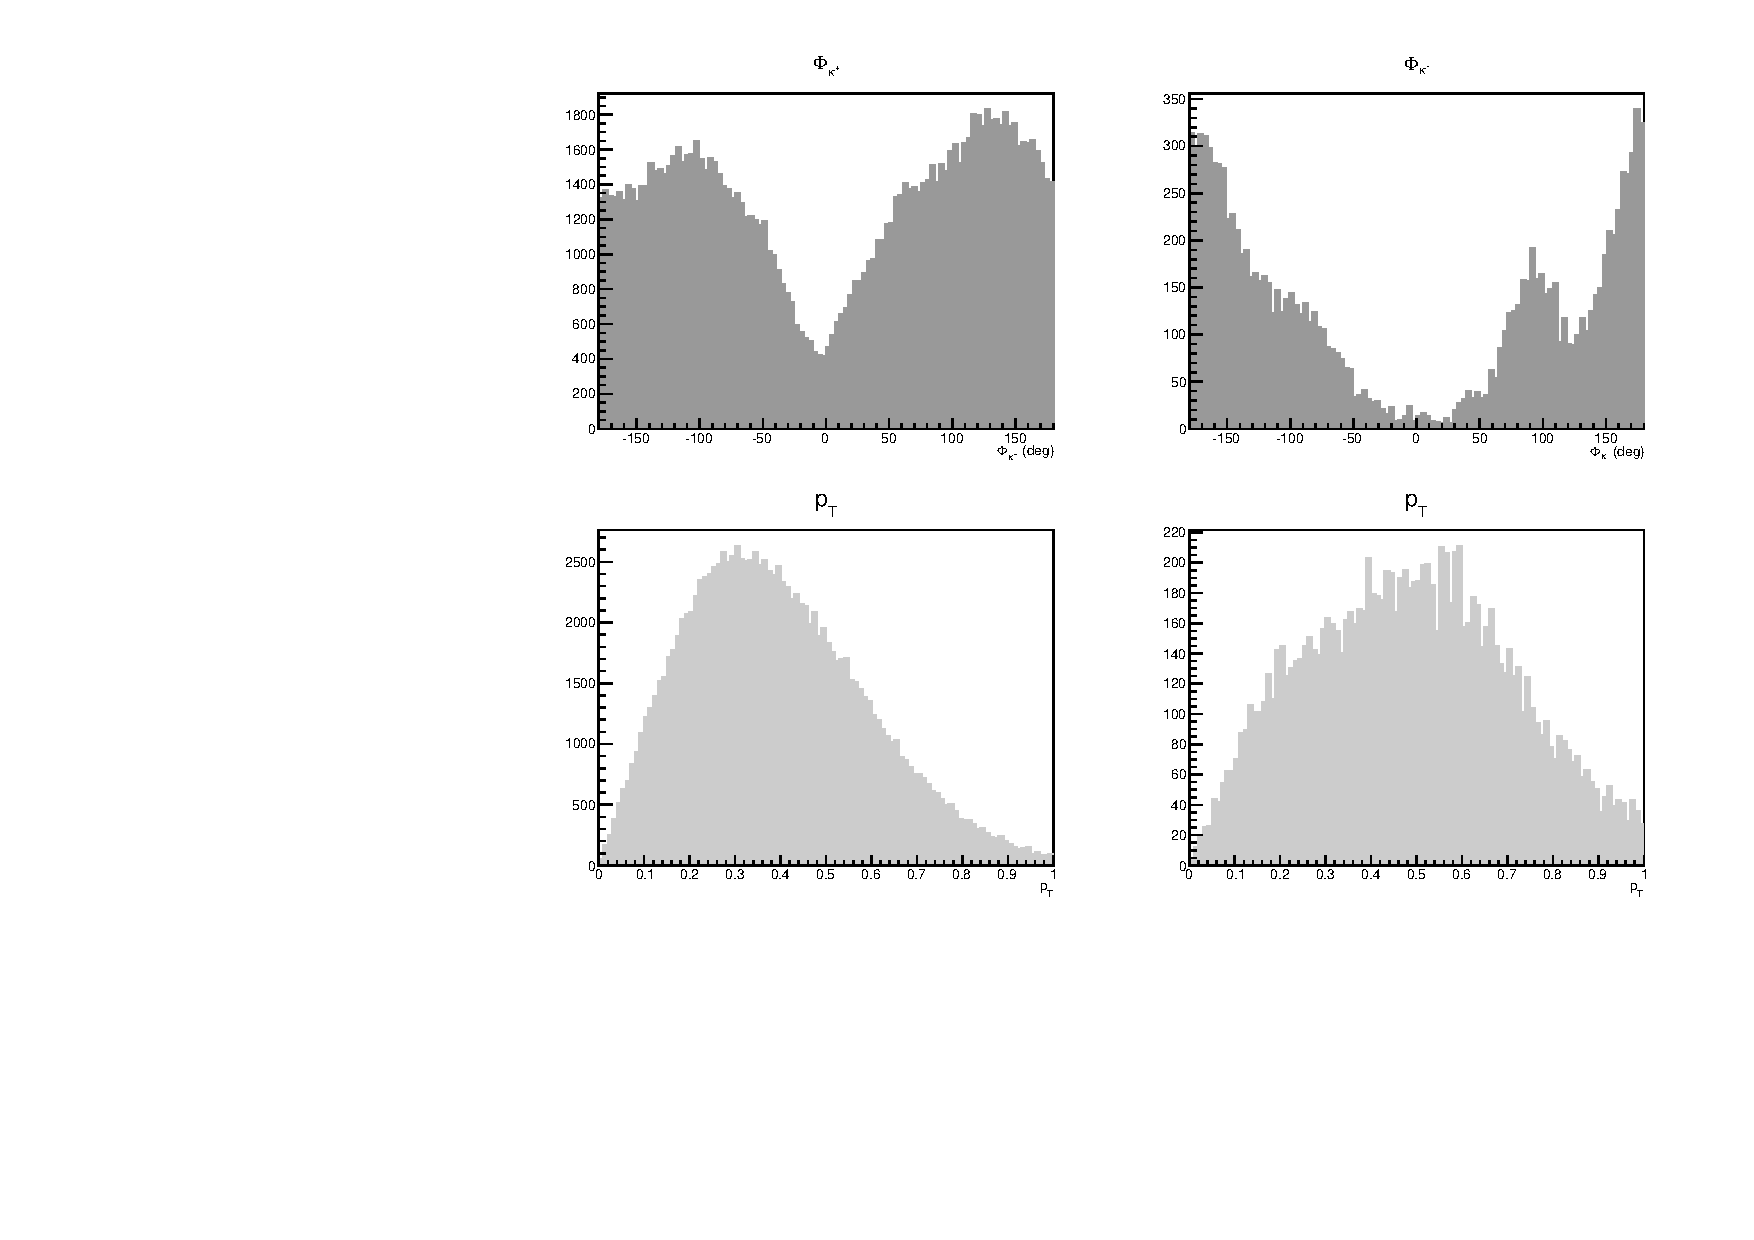
\includegraphics[width=1.0\textwidth]{sidis/phi_pt_kpm.pdf}
\caption{\label{fig::phi_pt_kpm} Definition of the angle $\phi$, formed by the leptonic and the hadronic planes.}
\end{figure}
%
%
%
\subsection{Projections}
%
The projections in this section are based on a full simulation of inclusive and semi-inclusive inelastic scattering with the CLAS12 acceptance folded in. Events were generated with the clas12DIS generator \cite{CLAS12DIS}, an implementation of the LUND Monte Carlo package PEPSI (Polarized Electron-Proton Scattering Interactions)~\cite{Mankiewicz:1991dp}. 
It is based on polarized and unpolarized parton distribution functions and the LUND string model for hadronization.
It has been tested successfully against several low-$Q^2$ experiments with 5.7-GeV beam at Jefferson Lab.\\

A fast Monte Carlo simulation program  has been used to define the acceptance and resolution of the CLAS12 detector with all of the standard (base) equipment
in place. The kaons were assumed identified 100\% in sectors covered by the CLAS12 RICH, and also at energies above 5 GeV, where the pions start to fire the High Threshold Cherekov Counter (HTCC).
The events generated by clas12DIS are used as input and all particles are followed through all detector elements. 
The results of this simulation have been cross-checked with direct cross-section calculations and a simple geometric acceptance model. The resolution of the detector is simulated by a simple smearing function which modifies a particle's track by a random amount in momentum and angles according to a Gaussian distribution of the appropriate width.
%The amount of smearing follows the design specifications of the CLAS12 detector. The resolution in $x_B$ varies between $0.01 < \sigma_{x} <  0.035$ and is therefore finer than our planned $x$ bin size of 0.05 in all cases.
%A full Monte Carlo simulation (GEANT-based) of CLAS12 with all resolution effects will be used to determine the effective mean $x$ (and $Q^2$) for each $x$-bin we will use to bin our data so we can accurately extract the $x$-dependence of the measured asymmetries.

%
\subsection{Expected results}
%
Kaon production being suppressed by an order of magnitude with respect to pion production, observables related to kaon production in DIS will benefit the most from the additional 50 days on a longitudinally polarized deuteron target requested in this proposal. Simultaneous measurements of the Kotzinian-Mulders asymmetry for pions and kaons on proton and deuteron targets will provide an independent measurement of ratios of their Collins functions, providing complementary measurements to the $e^+e^-$ ones. 
The extracted dependencies on $(x_B, Q^2, P_T, z)$ on both pions and kaons will provide access to widths in the transverse momentum of different underlying partonic distributions, like $g_1$ and $h_{1L}$, and to their flavor dependence. Proposed measurements can be used to test the evolution properties of the Collins function. They will also provide a check of chiral limit prediction, where the ratio of pion and kaon fragmentation functions is expected to be at unity.
%With the knowledge of the Collins function, one can study all involved TMD distributions.
Figures \ref{fig::ALLptcosdeutpionsx2} and \ref{fig::ALLptcosdeutkaonsx2} show the distributions of the double-spin asymmetry constant term on deuteron as a function of the hadron $p_T$, for pions and kaons respectively, for a total beam time of 100 days (the 50 already approved for Run Group C plus the 50 more requested in this Run-Group-extension proposal).
%The read and blue curves are calculations in constituent quark model [24] using
%Schlumpf’s wave function [62] and the hypercentral wave function for the momentum
%dependence of the light-cone wave function [63].
\textbf{add description of models}
While pion projections show already a reasonable discriminating power among the available models, kaon ones turned out to be barely sufficient to test the phenomenological accuracy of the models, especially in the high-$p_T$ region where the hadron acceptance drops (see Fig.~\ref{fig::phi_pt_kpm}). This affects in particular $k^-$, the rate of which is suppressed with respect to $k^+$.
The high-$p_T$ region is also the one less constrained from other measurements, and it would benefit the most from an increased statistics for the CLAS12 measurement.
%
% pions vs pt x2
\begin{figure}
\centering
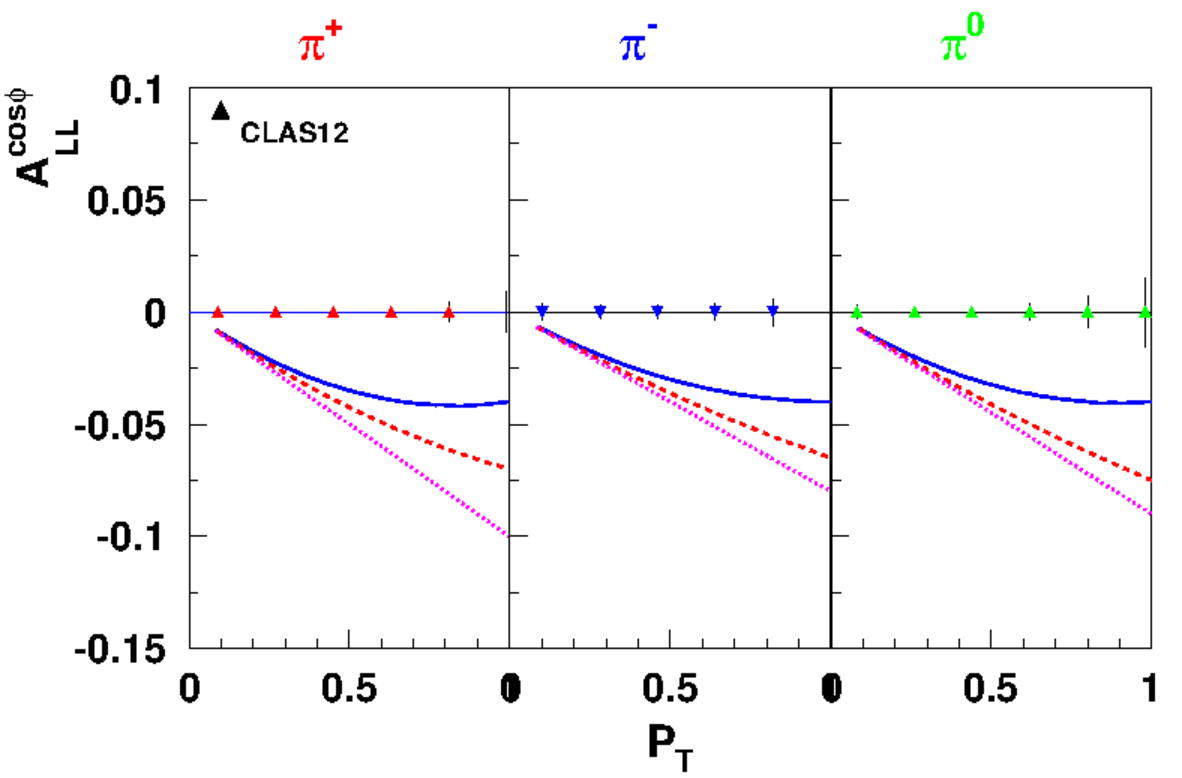
\includegraphics[width=1.0\textwidth]{sidis/all_pions_x2.pdf}
\caption{\label{fig::ALLptcosdeutpionsx2}$\cos\phi$ moment of the longitudinal double spin asymmetry for SIDIS kaon electroproduction, as a function of $p_T$. Left plot: positive pions; central plot: negative pions right plot: neutral pions.}
\end{figure}
%
% ALL kaons vs pt x2
\begin{figure}
\centering
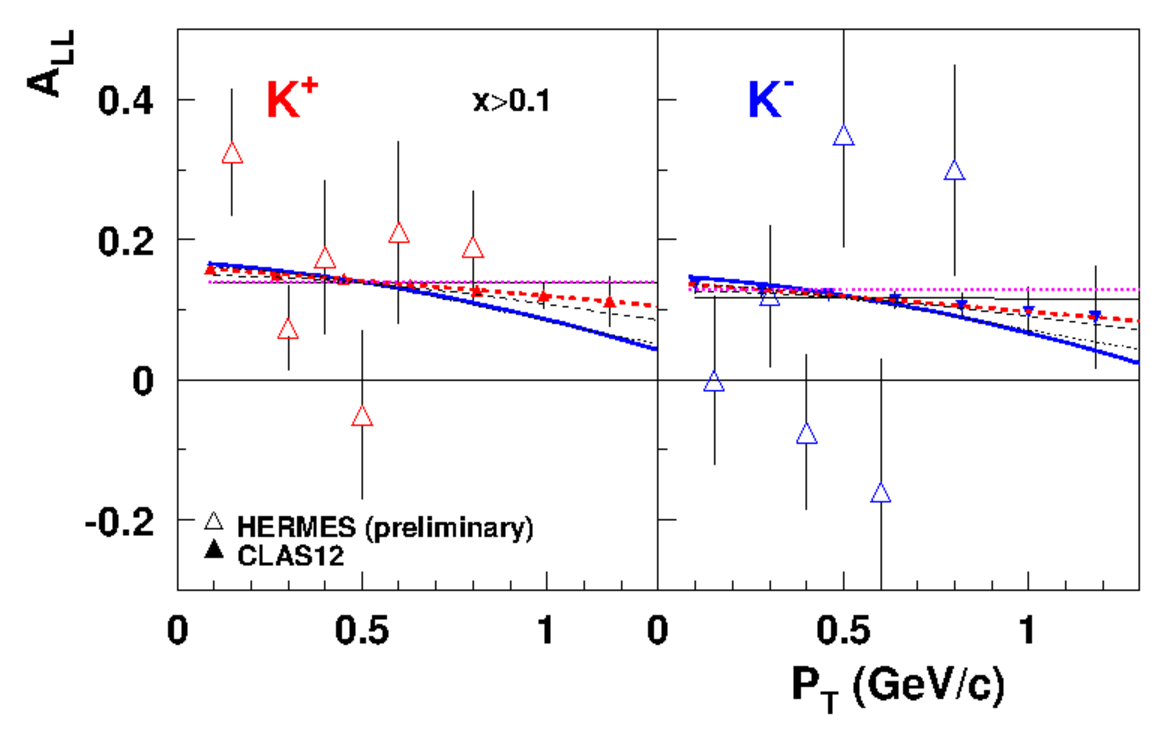
\includegraphics[width=1.0\textwidth]{sidis/all_kaons_x2.pdf}
\caption{\label{fig::ALLptcosdeutkaonsx2}$\cos\phi$ moment of the longitudinal double-spin asymmetry for SIDIS kaon electroproduction, as a function of $p_T$. Left plot: positive kaons; right plot: negative kaons.}
\end{figure}
%
%
The $\sin2\phi$ moment of the longitudinal target-spin asymmetry is shown in Fig.~\ref{fig::AULptcosdeutkaonsx2} as a function of $x_B$, for both positive (left) and negative (right) kaons. Projections in the high-$x_B$ region show the importance of an increased statistics, since it is where the present models are less constrained and differ the most in their prediction. 
The valence region is the main domain of CLAS12 physics, and it is mandatory to assure a reasonable statistical coverage for the relevant channels - as the semi-inclusive production of kaons - in this regime, not being accessible by the other experiments. 
%
% AUL kaons vs pt x2
\begin{figure}
\centering
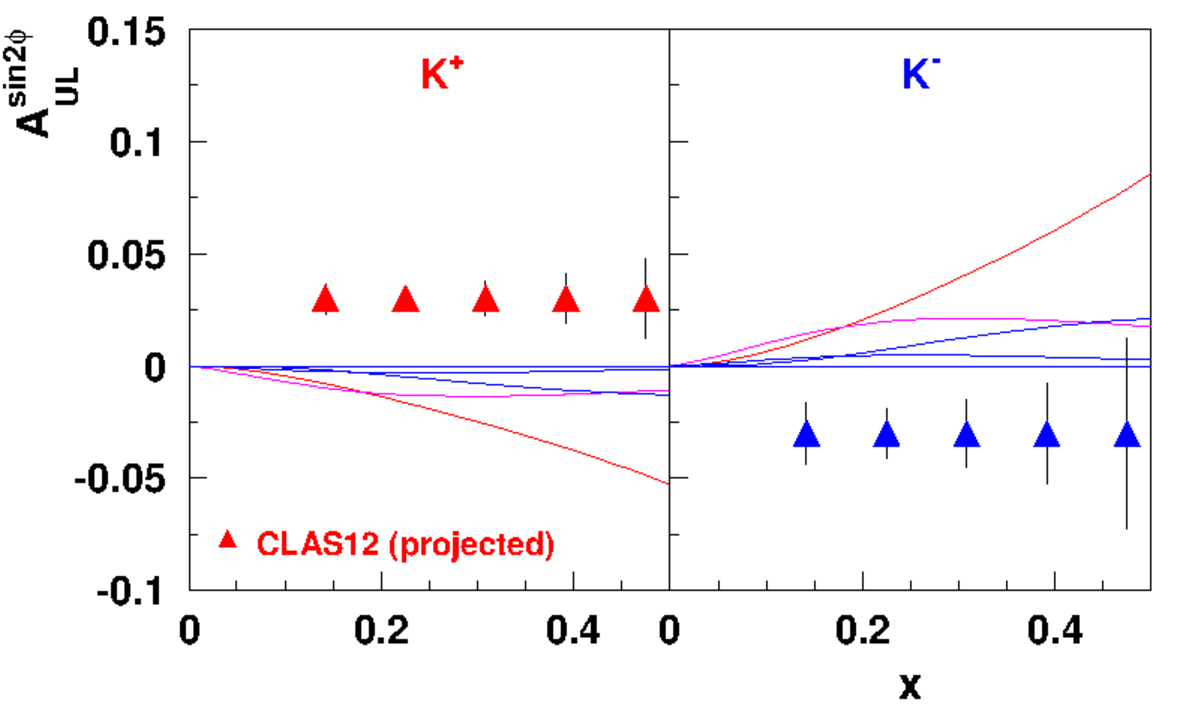
\includegraphics[width=1.0\textwidth]{sidis/aul_kaons_x2.pdf}
\caption{\label{fig::AULptcosdeutkaonsx2}$\sin\phi$ moment of the longitudinal target-spin asymmetry for SIDIS kaon electroproduction, as a function of $p_T$. Left plot: positive kaons; right plot: negative kaons.}
\end{figure}
%
%
\subsection{Semi-inclusive production of hadron pairs}
%
%
In addition to the semi-inclusive production of single hadrons, other semi-inclusive channels would benefit from an increased statistics on a longitudinally polarized deuteron target. 
In the last years, for example, an increasing role is being played by the SIDIS production of hadron pairs, which gives the cleanest access to the chiral-odd one-dimensional picture of the nucleon. Differently from the quark (unpolarized) and helicity 1D distribution functions, the transversity distribution, as well as the two higher-twist PDF $e(x)$ and $h_L(x)$, cannot be accessed through inclusive DIS. This is due to their \textit{chiral-odd} nature, that prevents the access through inclusive observables. In order to be accessed, indeed, they have to appear in the observables coupled to a second \textit{chiral-odd} function, the so-called Di-Hadron fragmentation functions. The latter are the analogous of the single hadron FF described earlier in the text, and encode the fragmentation of the struck quark to the final \texttt{hadron pair}. 
The main advantage of the di-hadron production is the fact that, while in the single-hadron case the distribution functions and the fragmentation functions appear coupled in the structure functions through a convolution integral, in the di-hadron case they are coupled through a simple product, making the final extraction easier and less sensitive to model assumptions. 
Among the chiral-odd PDFs, the higher-twist $h_L(x)$ is by far the least known. It can only be accessed through the di-hadron longitudinal target-spin asymmetry, where it appears coupled to the interference fragmentation functions $H_1^\sphericalangle$, that represents the analogous of the Collins function of the single-hadron case.
Together with $e(x)$, it opens the avenue to a deeper understanding of the quark-gluon-quark correlations inside the nucleon. No measurements of such an observable are presently available on a deuteron target. Preliminary analysis on a $NH_3$ target by CLAS shows a first non zero $A_{UL}$ on the proton. This preliminary observation would be greatly improved by a high-precision extraction in the extended kinematics accessible by CLAS12, both on a proton and on a deuteron target. A combined measurement of the di-hadron $A_{UL}$ on both proton and deuteron will be highly beneficial, since it will allow to perform the flavor separation of the PDFs and of the di-hadron FF. As for the single-hadron case, in order to properly disentangle the dependences of the PDF and the FF, a multidimensional mapping will be essential. Due to the reduced phase-space for the di-hadron case with respect to single hadron, an increased statistics will be essential to reach a proper accuracy in all the bins.
%
%
%
\begin{thebibliography}{}

\bibitem{Ji:2002aa} X.D. Ji and F. Yuan, Phys. Lett. B543, 66 (2002).
\bibitem{Ji:2002xn} X.D. Ji, J.P. Ma, and F. Yuan, Nucl. Phys. B652, 383  (2003). 
\bibitem{Belitsky:2002sm} A.V. Belitsky, X. Ji, and F. Yuan, Nucl. Phys. B656, 165 (2003).
\bibitem{Sivers:1990fh} D.W. Sivers, Phys. Rev. D. 43, 261 (1991). 
\bibitem{Anselmino:1998yz} M. Anselmino and F. Murgia, Phys. Lett. B442, 470 (1998). 
\bibitem{Brodsky:2002rv} S.J. Brodsky, D.S. Hwang, and I. Schmidt, Nucl. Phys. B 642, 344 (2002). 
\bibitem{Collins:2002kn} J.C. Collins, Phys. Lett. B536, 43 (2002). 
\bibitem{Mankiewicz:1991dp} L. Mankiewicz, A. Schafer, and M. Veltri,
 Comput. Phys. Commun. 71, 305 (1992). 
\bibitem{CLAS12DIS} H. Avakian and P. Bosted, "MC-generator for DIS studies with CLAS12" (2006)


\end{thebibliography}

%\end{document}
